%!TEX root = ../report.tex
\section{Elaborated Model}
In figure \ref{fig:system-context-diagram} the system architecture model is shown. This figure is an elaborated version of the system context figure in chapter 5.1. The arrows at the end of the lines represent data flows, going in that direction. 
First of all the system retrieves data from external API's. The data is retrieved by the data collection system and send to the database. The same applies for the UAV and sensor data. Besides this data flow, there is also a data flow from the data collection system to the UAV. In case the system detects that it needs UAV data, the data collection system sends commands to the UAV. The data collection system also retrieves the phone numbers and addresses of the citizens who have subscribed to the SMS service. After all data is collected the algorithm component will determine the flood probability based on the known data. If it detects that a flood is imminent, a warning message is sent to the warning system. This warning part then warns the emergency room by invoking the API. It also sends a text message to all the citizens that are in the affected area. To provide data to the third party applications the system holds an API. This API can be used by third party developers to get relevant data from the database. 
\begin{figure}[H]
\centering
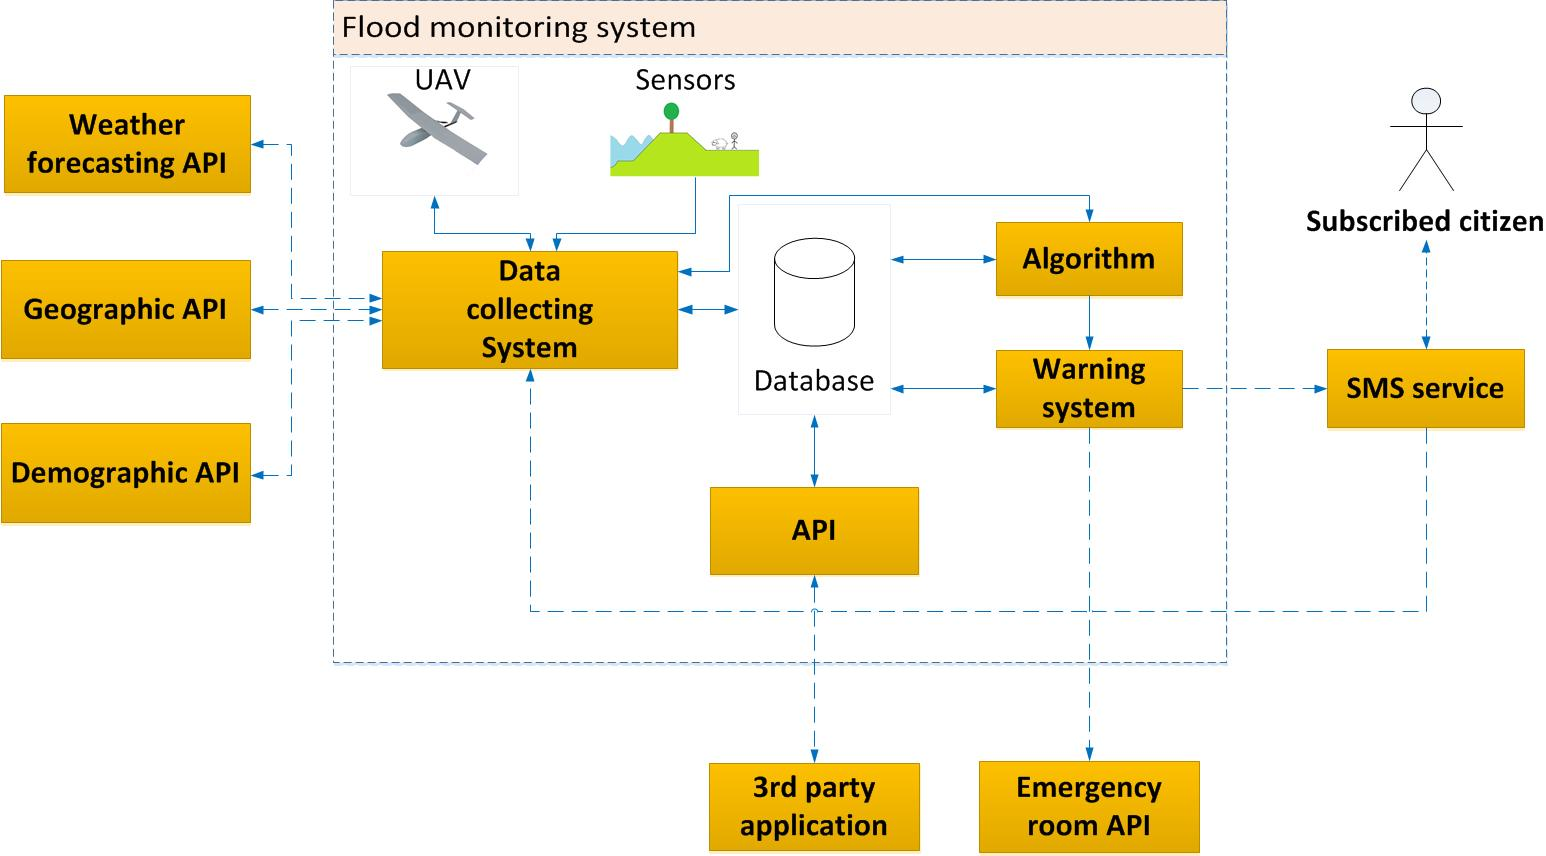
\includegraphics[keepaspectratio=true,width=1\textwidth]{images/Model_v3.jpg}
\caption{Elaborated system context diagram}
\label{fig:elaborated-model}
\end{figure}